\documentclass[UTF8]{article}

\usepackage{amsmath, amsfonts, amssymb, amstext, amscd, amsthm, bbm, CJKutf8, color, dsfont, enumerate, float, graphicx, hyperref, makeidx, mathrsfs, mathtools, marvosym, soul, url, verbatim, xcolor, xfrac}
\usepackage[left=2cm,top=2cm,right=2cm,bottom=2cm,bindingoffset=0cm]{geometry}
\allowdisplaybreaks 
\newenvironment{subproof}[1][Proof]
    {\proof[#1]\leftskip=1cm\rightskip=1cm}
	{\endproof}

%theorems with custom numbering
%\newtheorem{innerthm}{Theorem}
%\newenvironment{thm}[1]
    %{\renewcommand\theinnerthm{#1}\innercustomthm}
    %{\endinnerthm}

\newtheorem{theorem}{Theorem}
\newtheorem{lemma}{Lemma}
\newtheorem{proposition}{Proposition}
\newtheorem{corollary}{Corollary}
\newtheorem{claim}{Claim}
\newtheorem{conjecture}{Conjecture}
\newtheorem{justification}{Justification}
\newtheorem{definition}{Definition}
\newtheorem*{remark}{Remark}
\newtheorem*{note}{Note}

\renewcommand{\and}{\;\wedge\;}
\newcommand{\disj}{\;\vee\;}
\newcommand{\xor}{\;\oplus\;}
\newcommand{\divides}{\;|\;}
\newcommand{\suchthat}{\;\middle|\;}
\newcommand{\contradiction}{\;\text{\Large \Lightning}}
\newcommand{\conj}[1]{\overline{#1}}
\newcommand{\mean}[1]{\overline{#1}}
\newcommand{\integral}[1]{\smashoperator{\int_{#1}}}
\renewcommand{\restriction}[1]{\downharpoonright_{#1}}
\renewcommand{\qedsymbol}{QED} 
\DeclareMathOperator{\lcm}{lcm}
\DeclareMathOperator*{\argmin}{arg\!\min}
\DeclareMathOperator*{\argmax}{arg\!\max}

\let\originalleft\left
\let\originalright\right
\renewcommand{\left}{\mathopen{}\mathclose\bgroup\originalleft}
\renewcommand{\right}{\aftergroup\egroup\originalright}
\newcommand{\zh}[1]{\begin{CJK}{UTF8}{gbsn}#1\end{CJK}}
\newcommand{\jp}[1]{\begin{CJK}{UTF8}{gbsn}#1\end{CJK}}

\DeclarePairedDelimiterX \inner[2]{\langle}{\rangle}{#1,#2}
\DeclarePairedDelimiterX \braket[2]{\langle}{\rangle}{#1 \delimsize\vert #2}
\DeclarePairedDelimiter \bra{\langle}{\rvert}
\DeclarePairedDelimiter \ket{\lvert}{\rangle}
\DeclarePairedDelimiter \abs{\lvert}{\rvert}
\DeclarePairedDelimiter \lrangle{\langle}{\rangle}
\DeclarePairedDelimiter \norm{\lVert}{\rVert}
\DeclarePairedDelimiter \set{\lbrace}{\rbrace}
\DeclarePairedDelimiter \parens{(}{)}

\begin{document}
\begin{center}
	\textsc{\huge Applied Machine Learning}\\
	\textsc{\Large Homework 8}\\
\end{center}
\begin{flushright}
	Daniel Gonzalez\\
    Colton Piper\\
	$31^{\text{th}}$ of October, $2018$
\end{flushright}


\section{Results}

\subsection{Table}

\begin{table}[H]
\centering
    \caption{Summary of Results: Original Learning Rates}
    \begin{tabular}{|l|l|l|l|}
        \hline
        Data Set & Iteration $k$ & Training Error \% & Test Error \%\\\hline\cline{1-4}
        & $10$ & $7.467$ & $8.7$\\\cline{2-4}
        \texttt{gisette} & $30$ & $3.367$ & $3.8$\\\cline{2-4}
        & $100$ & $1.25$ & $3.0$\\\cline{2-4}
        & $300$ & $0.0$ & $2.7$\\\hline\cline{1-4}

        & $10$ & $7.333$ & $10.667$\\\cline{2-4}
        \texttt{dexter} & $30$ & $0.333$ & $9.333$\\\cline{2-4}
        & $100$ & $0.0$ & $9.0$\\\cline{2-4}
        & $300$ & $0.0$ & $8.333$\\\hline\cline{1-4}

        & $10$ & $37.7$ & $40.333$\\\cline{2-4}
        \texttt{madelon} & $30$ & $34.5$ & $42.833$\\\cline{2-4}
        & $100$ & $30.9$ & $43.333$\\\cline{2-4}
        & $300$ & $26.950$ & $43.167$\\\hline\cline{1-4}
\end{tabular}
\end{table}

\subsection{Figures}
\subsubsection{Misclassification Errors}
\begin{figure}[H]
    \centering
    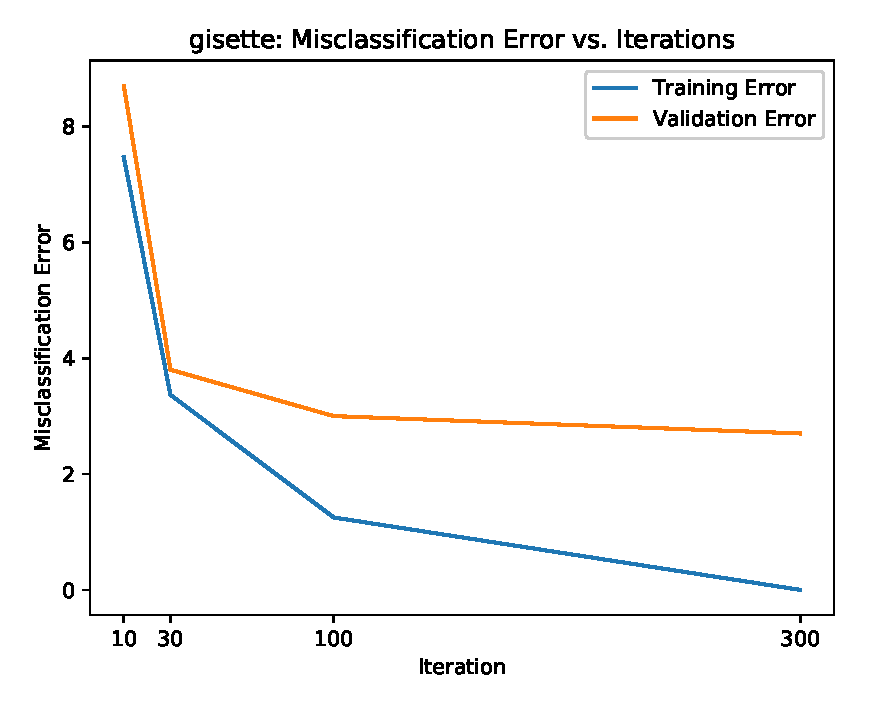
\includegraphics[scale=0.9]{./figures/gisette-error.eps}
\end{figure}
\begin{figure}[H]
    \centering
    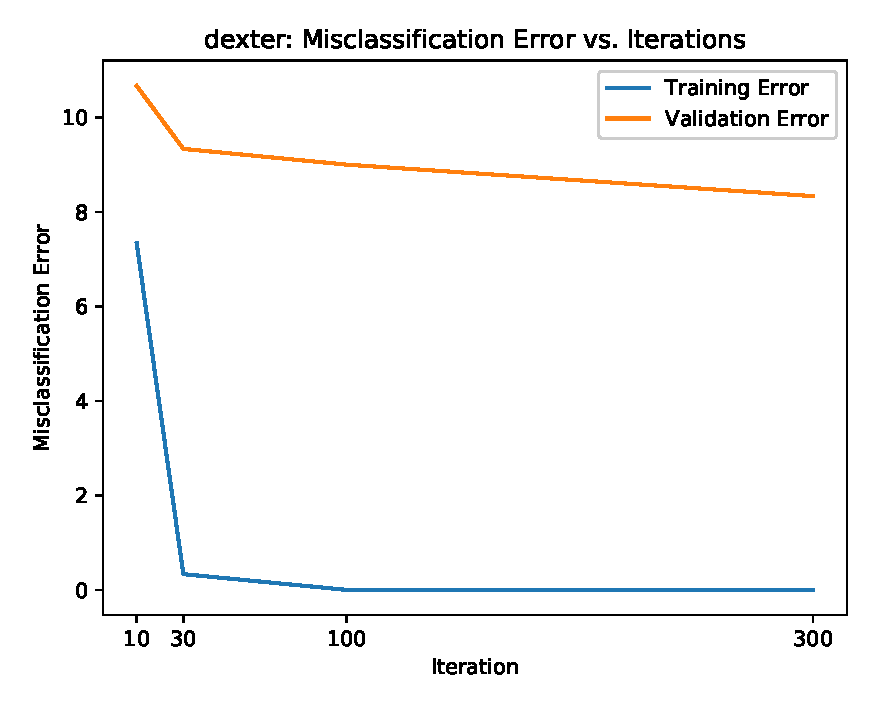
\includegraphics[scale=0.9]{./figures/dexter-error.eps}
\end{figure}
\begin{figure}[H]
    \centering
    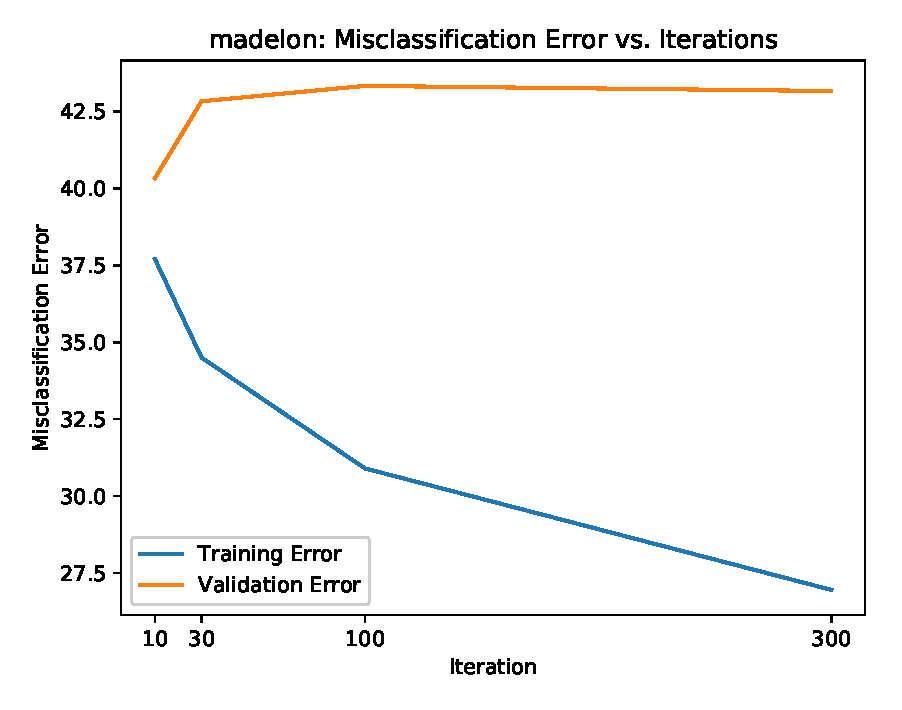
\includegraphics[scale=0.9]{./figures/madelon-error.eps}
\end{figure}

\subsubsection{Training Losses}
\begin{figure}[H]
    \centering
    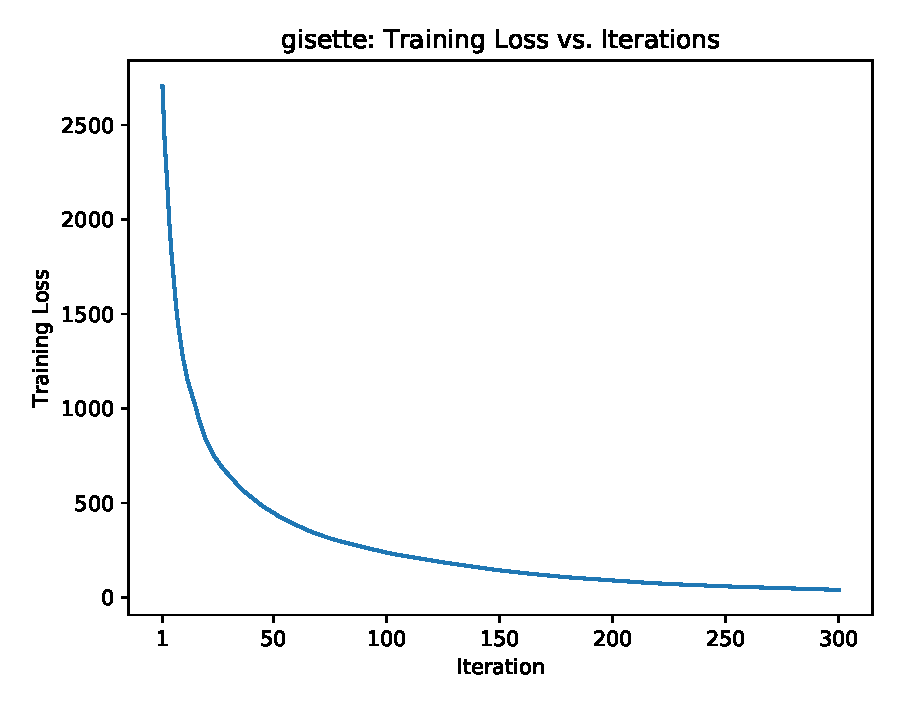
\includegraphics[scale=0.9]{./figures/gisette-loss.eps}
\end{figure}
\begin{figure}[H]
    \centering
    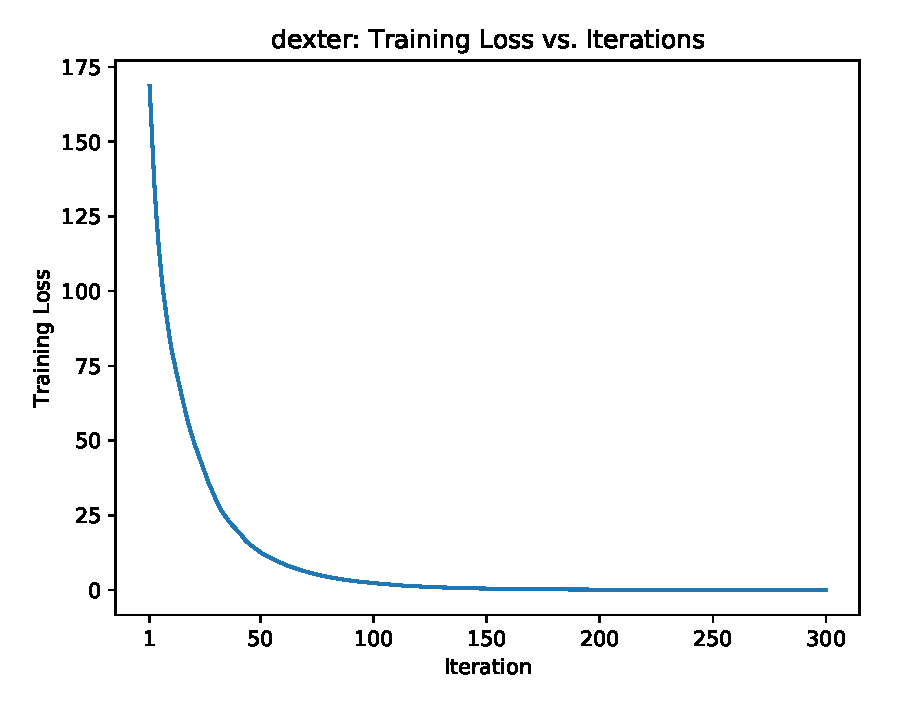
\includegraphics[scale=0.9]{./figures/dexter-loss.eps}
\end{figure}
\begin{figure}[H]
    \centering
    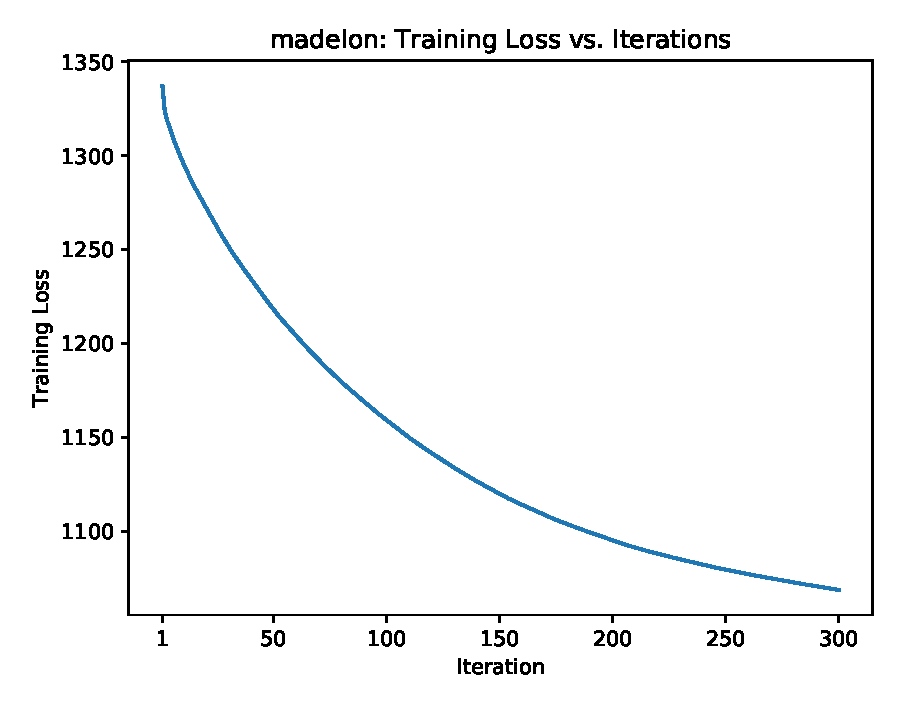
\includegraphics[scale=0.9]{./figures/madelon-loss.eps}
\end{figure}

\newpage
\section{Appendix: Code}
If the code looks too small, please zoom in on the pdf.
The screenshots are \texttt{.png} images, so you should be able to zoom in and read at whatever is a comfortable size for you.
The first two screenshots are of the actual FSA code, while the last screenshot is the python code for normalizing and pre-processing the data.
\begin{figure}[H]
    \centering
    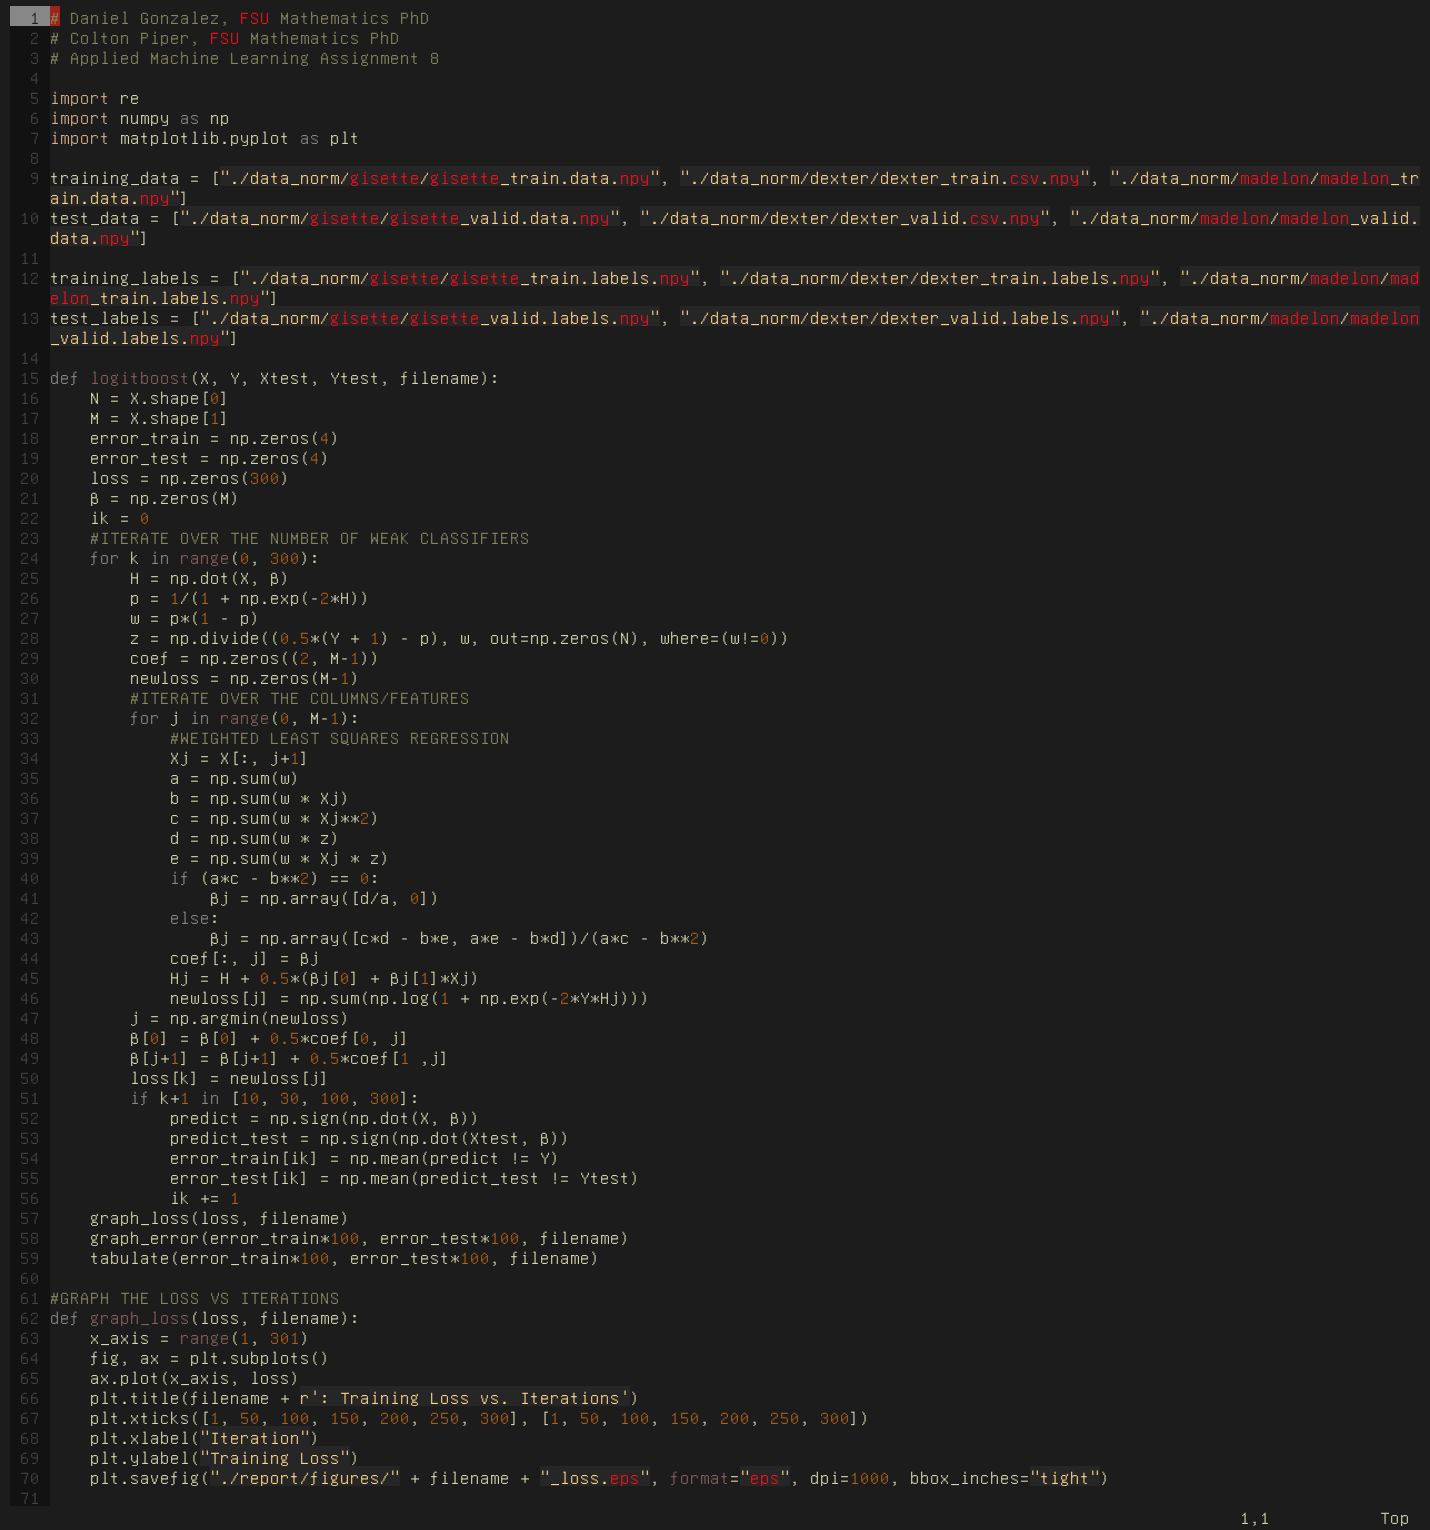
\includegraphics[scale=0.7]{./figures/code1.png}
\end{figure}
\begin{figure}[H]
    \centering
    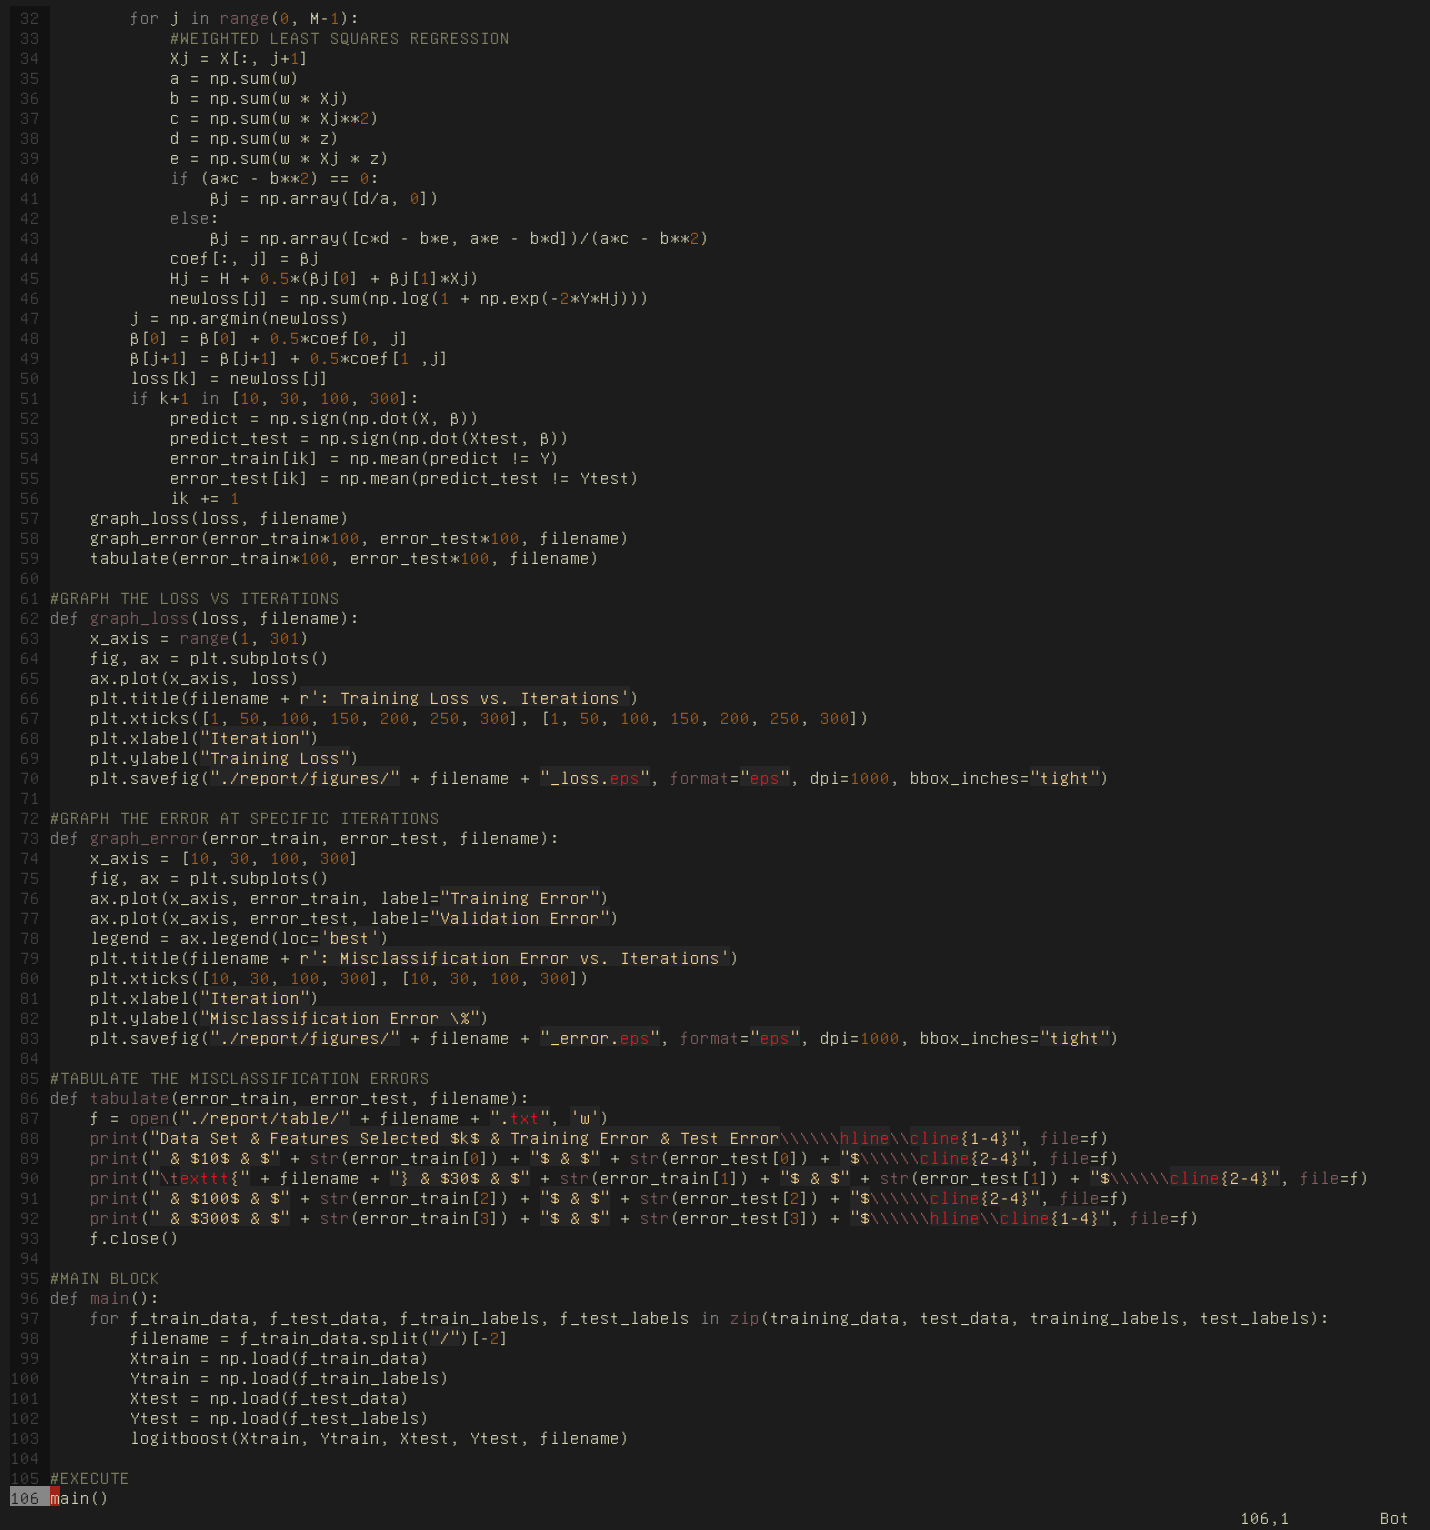
\includegraphics[scale=0.7]{./figures/code2.png}
\end{figure}
\begin{figure}[H]
    \centering
    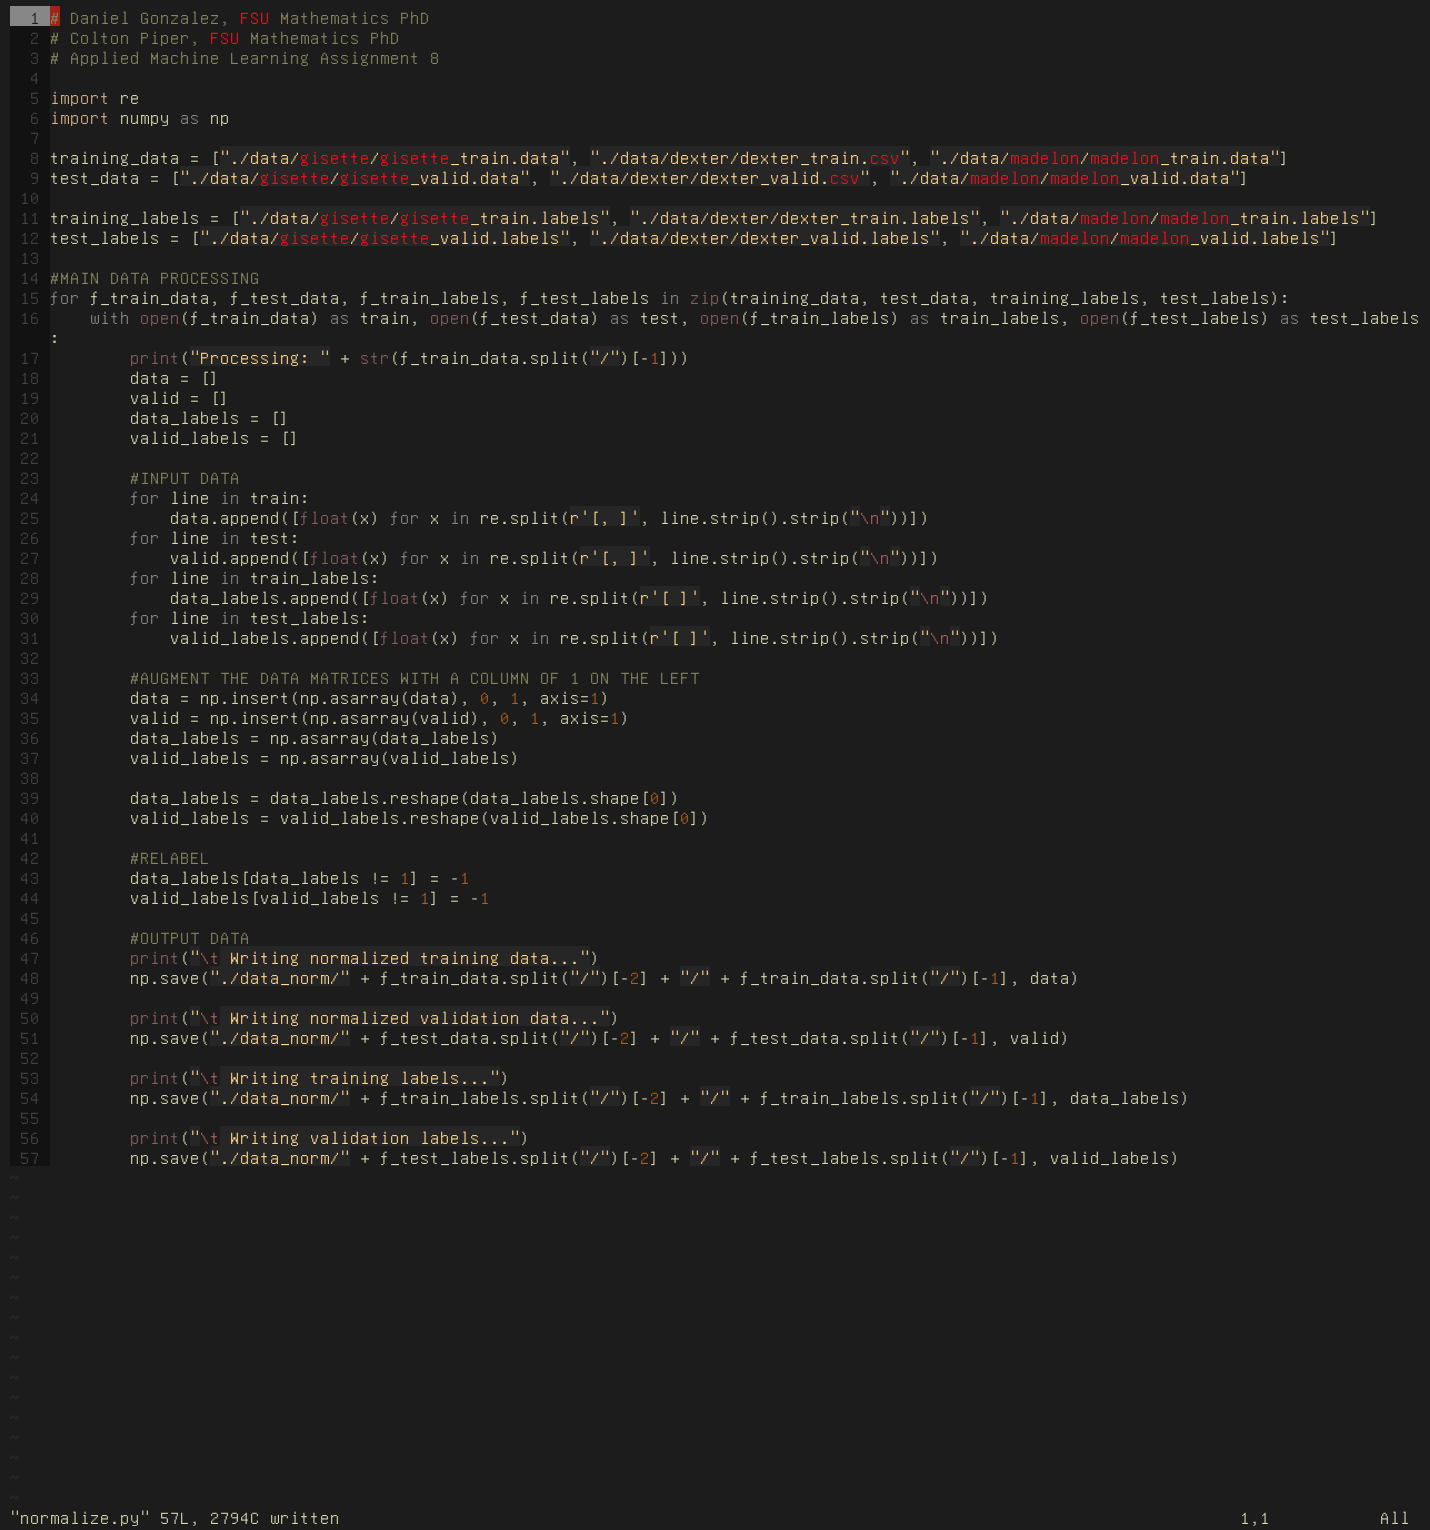
\includegraphics[scale=0.7]{./figures/code-norm.png}
\end{figure}

\end{document}
